\graphicspath{{02_massimi_e_minimi/figures/PNG/}{02_massimi_e_minimi/figures/PDF/}{02_massimi_e_minimi/figures/}}

\chapter{Massimi e minimi per funzioni di più variabili}
\copyrightnotice
\section{Il Teorema di Fermat}
\begin{definition}
Siano $A \subseteq \mathbb{R}^n$, $f : A \longrightarrow \mathbb{R}$.
\begin{enumerate}[labelindent=\parindent,leftmargin=*,label=\textnormal{(\roman*)},start=1]
\item Un punto $P_0 \in A$ si dice \emph{punto di minimo relativo (o locale)} [rispettivamente \emph{punto di massimo relativo (o locale)}] se $\exists \, r_0 > 0$ tale che
$$
f(P_0) \underset{[\geq]}{\leq} f(P) \qquad \forall \, P \in A \cap \mathrm{B}(P_0,\,r_0)
$$
\item Un punto $P_0 \in A$ si dice \emph{punto di minimo (assoluto o globale)} [rispettivamente \emph{punto di massimo relativo (assoluto o globale)}] se
$$
f(P_0) \underset{[\geq]}{\leq} f(P) \qquad \forall \, P \in A
$$
\end{enumerate}
Si definiscono, se esistono,
$$
\underset{A}{\mathrm{max}}f \overset{def}{=} \mathrm{max} \lbrace f(P) : P \in A \rbrace
$$
$$
\underset{A}{\mathrm{min}}f \overset{def}{=} \mathrm{min} \lbrace f(P) : P \in A \rbrace
$$
Se esistono, $\underset{A}{\mathrm{max}}f$ e $\underset{A}{\mathrm{min}}f$ sono unici. Si definiscono inoltre
$$
\underset{A}{\mathrm{sup}}f \overset{def}{=} \mathrm{sup} \lbrace f(P) : P \in A \rbrace
$$
$$
\underset{A}{\mathrm{inf}}f \overset{def}{=} \mathrm{inf} \lbrace f(P) : P \in A \rbrace
$$
$\underset{A}{\mathrm{sup}}f$ e $\underset{A}{\mathrm{inf}}f$ esistono sempre per l'Assioma di Completezza dei reali.
\end{definition}

\begin{thm}[di Fermat]
Siano $A \subseteq \mathbb{R}^n$, $f : A \longrightarrow \mathbb{R}$. Supponiamo che, dato $P_0 \in A$,
\begin{enumerate}[labelindent=\parindent,leftmargin=*,label=\textnormal{(\roman*)},start=1]
\item $P_0$ sia un punto di massimo o minimo relativo di $f$ su $A$.
\item $\exists \, \nabla f(P_0)$.
\item $P_0$ sia un punto interno di $A$, cioè $\exists r_0 > 0$ tale che $\mathrm{B}(P_0,\,r_0) \subseteq A$\footnote{Se $P_0$ non fosse interno, si avrebbero dei problemi. Ad esempio ($n=1$), se $A=[0,\,1]$ e $f(x)=x$, allora $x_0=0$ è un punto di minimo relativo, ma $f'(x_0) = 1 \neq 0$.}.
\end{enumerate}
Allora
$$\nabla f(P_0) = \underline{0} = (0,\ldots,0)$$
\end{thm}
\begin{proof}
\begin{center}
\def\svgwidth{8cm}
\input{./02_massimi_e_minimi/figures/fermat.pdf_tex}
\end{center}
Fissato $i=1,\ldots,n$, poiché $P^0$ è interno, $P^0 + he_i \in \mathrm{B}(P^0,\,r_0)$ se $|h| \leq r_0$. Definiamo
$$
F : (-r_0,\,r_0) \longrightarrow \mathbb{R}, \qquad F(h) = f(P^0+he_i)
$$
(Per $h=0$, $F(h)$ è interno!)\\
Applicando il teorema di Fermat in una variabile\footnote{
\cite{Greco2012}
Sia $f$ una funzione numerica, e $\overline{x}$ un punto di massimo locale (o minimo locale) di $f$. Se $\overline{x}$ è interno al dominio di $f$ ed $f$ è derivabile in $\overline{x}$, allora
$$f'(\overline{x}) = 0$$
}
, otteniamo che:
$$
\begin{array}{ccc}
\exists \, F'(0) &= 0 & \\
\rotatebox{90}{$\doteqdot$} & & \\
\displaystyle \frac{\partial f}{\partial x_i} (P^0) & & \qquad \forall \, i = 1,\,2,\ldots,n \\
\end{array}
$$
\end{proof}

\begin{definition}
Dati $A \subseteq \mathbb{R}^n$ e $f : A \longrightarrow \mathbb{R}$, si chiamano \emph{punti stazionari (o critici) liberi} di $f$ su $A$ i punti $P^0 \in A$ tali che:
\begin{enumerate}[labelindent=\parindent,leftmargin=*,label=\textnormal{(S\arabic*)},start=1]
\item $\exists \, \nabla f(P)$
\item $\nabla f(P) = \underline{0}$
\end{enumerate}
\end{definition}

\begin{example}
$f : \mathbb{R}^2 \longrightarrow \mathbb{R}$, $f(x,\,y) = x^2-y^2$.
Poniamo il gradiente di $f$ uguale a $0$ per trovare i punti stazionari:
$$
\nabla f(x,\,y) = 2(x,\,-y) = (0,\,0) \Longleftrightarrow x=y=0
$$
$P_0 = (0,\,0)$ è quindi un punto di minimo o massimo relativo di $f$? \underline{NO!}

Basta studiare il segno di $f(x,\,y) = x^2-y^2 = (x-y)(x+y)$ in un intorno di $(0,\,0)$ per accorgersi che non è così:
\begin{center}
\def\svgwidth{8cm}
\input{./02_massimi_e_minimi/figures/esempio_max.pdf_tex}
\end{center}
La funzione non è definitivamente positiva o negativa, come dovrebbe essere nel caso di un punto di massimo o di minimo! In particolare, in questo caso si dice che il punto è di \emph{sella}.
\end{example}

\begin{definition}
Sia $H = (h_{ij})_{n \times n}$ a coefficienti reali (cioè $h_{ij} \in \mathbb{R} \quad \forall \, i,\,j = 1,\ldots,n$).
\begin{enumerate}[labelindent=\parindent,leftmargin=*,label=\textnormal{(\roman*)},start=1]
\item $H$ si dice \emph{definita positiva} se 
$\left( Hv \bullet v \right) > 0 \qquad \forall v \in \mathbb{R}^n \setminus \lbrace 0 \rbrace$
\item $H$ si dice \emph{definita negativa} se 
$\left( Hv \bullet v \right) < 0 \qquad \forall v \in \mathbb{R}^n \setminus \lbrace 0 \rbrace$
\item $H$ si dice \emph{semidefinita positiva} se 
$\left( Hv \bullet v \right) \geq 0 \qquad \forall v \in \mathbb{R}^n \setminus \lbrace 0 \rbrace$
\item $H$ si dice \emph{semidefinita negativa} se 
$\left( Hv \bullet v \right) \leq 0 \qquad \forall v \in \mathbb{R}^n \setminus \lbrace 0 \rbrace$
\end{enumerate}
\end{definition}

\begin{lemma}[Criterio per i segni di una matrice quadrata simmetrica]
Sia $H = (h_{ij})_{n \times n}$ simmetrica (cioè, per definizione, $h_{ij} = h_{ji} \quad \forall \, i,\,j = 1,\ldots,n$). Allora definiamo come:\\
\indent $m \overset{def}{=}$ ``il più piccolo autovalore di $H$''\\
\indent $M \overset{def}{=}$ ``il più grande autovalore di $H$''\\
Allora
\begin{center}
$\mathrm{(\star)}$
\hfill
$\displaystyle
m||v||_n^2 \leq Hv \bullet v \leq M||v||_n^2$
\hfill \null \\
\end{center}
Da $\mathrm{(\star)}$ e dalla definizione, segue che:
\begin{enumerate}[labelindent=\parindent,leftmargin=*,label=\textnormal{(\roman*)},start=1]
\item $H \text{ è definita positiva } \quad \Longleftrightarrow \quad m > 0$
\item $H \text{ è definita negativa } \quad \Longleftrightarrow \quad M < 0$
\item $H \text{ è semidefinita positiva } \quad \Longleftrightarrow \quad m \geq 0$
\item $H \text{ è semidefinita negativa } \quad \Longleftrightarrow \quad M \leq 0$
\end{enumerate}
\end{lemma}

\begin{thm}
Siano $A \subseteq \mathbb{R}^n$, $f : A \longrightarrow \mathbb{R}$, e supponiamo che $f \in C^2(A)$. Sia ora $x^0 \in A$ un punto stazionario (libero) di $f$ su $A$, cioè, per definizione, $\nabla f (x^0) = \underline{0}$. Prendiamo inoltre la matrice $\displaystyle H(f)(x^0) = \left( \frac{\partial^2 f}{\partial x_i \partial x_j} (x^0) \right)_{n \times n}$, detta \emph{matrice hessiana} di $f$ nel punto $x^0$. Allora
\begin{enumerate}[labelindent=\parindent,leftmargin=*,label=\textnormal{(\roman*)},start=1]
\item Se $H(f)(x^0)$ è definita positiva $\quad \Longrightarrow \quad$ $x^0$ è un punto di \emph{minimo relativo} di $f$ su $A$
\item Se $H(f)(x^0)$ è definita negativa $\quad \Longrightarrow \quad$ $x^0$ è un punto di \emph{massimo relativo} di $f$ su $A$
\item Se $x^0$ è un punto di minimo relativo di $f$ su $A$ $\quad \Longrightarrow \quad$ $H(f)(x^0)$ è semidefinita positiva
\item Se $x^0$ è un punto di massimo relativo di $f$ su $A$ $\quad \Longrightarrow \quad$ $H(f)(x^0)$ è semidefinita negativa
\end{enumerate}
\end{thm}
\begin{proof}
\begin{enumerate}[labelindent=\parindent,leftmargin=*,label=\textnormal{(\roman*)},start=1]
\item ($\underline{n=2}$)\\
\begin{center}
\def\svgwidth{8cm}
\input{./02_massimi_e_minimi/figures/thm_min_i.pdf_tex}
\end{center}
Essendo $A$ aperto, $\exists \, r_0 > 0$ tale che $\mathrm{B}(x^0,\,r_0) \subset A$, e quindi $f \in C^2 \left( \mathrm{B}(x^0,\,r_0) \right)$. Applicando la formula di Taylor al \RNum{2} ordine, cioè $\mathrm{(FT_2)}$, otteniamo che:
\begin{center}
$\mathrm{(1)}$
\hfill
$\displaystyle
f(x) = f(x^0) + df(x^0)(x-x^0) + \frac{1}{2} \left( H(f)(x-x^0) \bullet (x-x^0) \right) + R_2(x,\,x^0)
$
\hfill \null \\
\end{center}
tale che
\begin{center}
$\mathrm{(2)}$
\hfill
$\displaystyle
\exists \, \lim_{x \rightarrow x^0} \frac{R_2(x,\,x^0)}{||x-x^0||_n^2} = 0
$
\hfill \null \\
\end{center}
Essendo $x^0$ un punto stazionario di $f$, vale:
$$
df(x^0)(x-x^0) = \nabla f(x^0) \bullet (x-x^0) = 0
$$
Dunque possiamo riscrivere la $\mathrm{(1)}$ nel modo seguente:
\begin{center}
$\mathrm{(3)}$
\hfill
$\displaystyle
f(x) - f(x^0) = \frac{1}{2} \left( H(f)(x-x^0) \bullet (x-x^0) \right) + R_2(x,\,x^0)
$
\hfill \null \\
\end{center}
Sia $m$ il più piccolo degli autovalori di $H(f)(x^0)$. Da $\mathrm{(\star)}$, prendendo $H = H(f)(x^0)$, ottengo che:
\begin{center}
$\mathrm{(4)}$
\hfill
$\displaystyle
f(x) - f(x^0) \geq \frac{m}{2} ||x-x^0||_n^2 + R_2(x,\,x^0)
$
\hfill \null \\
\end{center}
ed $ m > 0$, essendo $H(f)(x^0)$ definita positiva.

Dalla $\mathrm{(2)}$, usando la definizione e scegliendo $\varepsilon = \frac{m}{2} > 0, \quad \exists \; 0 < r_1 < r_0$ tale che:
\begin{center}
$\mathrm{(5)}$
\hfill
$\displaystyle
-\frac{m}{2} < \frac{R_2(x,\,x^0)}{||x-x^0||_n^2} < \frac{m}{2} \qquad \forall x \in \mathrm{B}(x^0,\,r_1) \setminus \lbrace x^0 \rbrace
$
\hfill \null \\
\end{center}
Da $\mathrm{(4)} + \mathrm{(5)}$ (moltiplicando $\mathrm{(5)}$ per $||x-x^0||_n^2$), segue che
\begin{center}
$\mathrm{(6)}$
\hfill
$\displaystyle
\begin{array}{rcl}
f(x) - f(x^0) & \geq & \frac{m}{2}||x-x^0||_n^2 - \frac{m}{2}||x-x^0||_n^2 \qquad \forall x \in \mathrm{B}(x^0,\,r_1)\\ 
& \big\lvert & \\
& \geq & 0
\end{array}
$
\hfill \null \\
\rotatebox{270}{$\overset{def}{\Longleftrightarrow}$} \\
$x^0$ è un punto stazionario di minimo relativo di $f$ su $A$
\end{center}

\item Si dimostra similmente al punto precedente, definendo $M$ il più grande degli autovalori di $H(f)(x^0)$ e applicando poi la $\mathrm{(\star)}$.

\item Prendiamo la direzione $v \in \mathbb{R}^n \setminus \lbrace 0 \rbrace$ (ricordiamo che, poiché $v$ è una direzione, $||v||_n = 1$).
\begin{center}
\def\svgwidth{8cm}
\input{./02_massimi_e_minimi/figures/thm_min_iii.pdf_tex}
\end{center}
Definiamo
$$
F(t) = f(x^0 + tv) \qquad \text{se} \qquad |t| \leq \delta
$$
(ossia $f$ ristretta ad una direzione).

Osserviamo che, essendo $A$ aperto, $F$ è ben definita se $\delta$ è abbastanza piccolo. Per ipotesi, $t = 0$ è un punto di minimo relativo di $F : [-\delta,\,\delta] \longrightarrow \mathbb{R}$ con
$$
F = f \circ g
$$
dove $g : [-\delta,\,\delta] \longrightarrow A$ tale che $g(t) = x^0 + tv$, quindi:
$$
F''(0) \geq 0
$$
Nella dimostrazione del Teorema di Fermat, avevamo già calcolato che:
$$
F^{(k)}(t) = 
\sum_{i_1=1,\ldots,i_k=1}^2
\frac{\partial^k f}{\partial x_{i_1} \ldots \partial x_{i_k}}(x^0+t(x-x^0))
(x_{i_1}-x_{i_1}^0) \ldots (x_{i_k}-x_{i_k}^0)
$$
Nel nostro caso, la formula diventa:
$$
F^{(2)}(0) = 
\sum_{i_1=1,\,i_2=1}^2
\frac{\partial^2 f}{\partial x_{i_1} \partial x_{i_2}}(x^0)
(x_{i_1}-x_{i_1}^0)(x_{i_2}-x_{i_2}^0) =
H(f)(x^0)v \bullet v
$$
con $v = (x-x^0)$. Dunque, $\forall \, v \in \mathbb{R}^n \setminus \lbrace 0 \rbrace$,
$$
H(f)(x^0)v \bullet v \geq 0
$$
\end{enumerate}
\end{proof}

\begin{exer}[Ex. 5, Foglio 5]
Determinare i massimi e i minimi relativi della funzione
$$
f(x,\,y) \doteqdot x^2 + 2kxy + y^2, \qquad (x,\,y) \in \mathbb{R}^2
$$
al variare del parametro $k \in \mathbb{R}$.
\end{exer}
\begin{proof}
Osserviamo che $f \in C^2(\mathbb{R}^2)$ (in effetti, $f \in C^{\infty}(\mathbb{R}^2)$). I punti stazionari liberi di $f$ sono dati dall'equazione:
$$
\nabla f(x,\,y) = (0,\,0)
$$
ossia, sviluppando,
$$
(2x + 2ky ,\, 2kx + 2y) = 2(x + ky ,\, kx + y) = (0,\,0)
$$
$$
\Updownarrow
$$
$$
\begin{cases}
x+ky=0\\
kx+y=0
\end{cases}
$$
Scriviamo la matrice associata al sistema e risolviamo:
$$
\left(
\begin{array}{cc|c}
1 & k & 0\\
k & 1 & 0
\end{array}
\right)
\Longleftrightarrow
\begin{array}{c}
\\
\RNum{2} - k\RNum{1}
\end{array}
\left(
\begin{array}{cc|c}
1 & k & 0\\
0 & 1-k^2 & 0
\end{array}
\right)
$$
Discutiamo i casi che ci si presentano:
\begin{itemize}
\item \underline{$k \neq 1$:} Il sistema ammette soluzione unica $(0,\,0)$.
\item \underline{$k = \pm 1$:} Il sistema ammette infinite soluzioni, generate dai vettori $\left( \begin{array}{c}
1\\1
\end{array} \right)$
e
$\left( \begin{array}{c}
-1\\1
\end{array} \right)$.
\end{itemize}
Andiamo ora a calcolare $H = H(f)(x,\,y) =$
$$
=
\left(
\begin{array}{cc}
\frac{\partial^2 f}{\partial x^2} (x,\,y) & \frac{\partial^2 f}{\partial x \partial y} (x,\,y)\\
\frac{\partial^2 f}{\partial y \partial x} (x,\,y) & \frac{\partial^2 f}{\partial y^2} (x,\,y)
\displaystyle 
\end{array}
\right)
=
\left(
\begin{array}{cc}
2 & 2k\\
2k & 2
\end{array}
\right)
$$
Quindi, calcoliamo gli autovalori di $H$ secondo la definizione:
$$
\mathrm{det}(H-\lambda I)=0
\Longleftrightarrow
\mathrm{det} \left(
\begin{array}{cc}
2-\lambda & 2k\\
2k & 2-\lambda
\end{array}
\right)=0
\Longleftrightarrow
(2-\lambda)^2-4k^2 = 0
\Longleftrightarrow
$$
$$
\Longleftrightarrow
(2-\lambda-2k)(2-\lambda+2k)=0
$$
e in definitiva:
$$
\begin{cases}
\lambda_{1} = 2-2k\\
\lambda_{2} = 2+2k
\end{cases}
$$
Ne deduciamo che:
\begin{itemize}
\item Se $|k|>1, \quad \lambda_{1}\lambda_{2} < 0 \quad$ e quindi
	\begin{itemize}
	\item $H$ non è né semidefinita positiva né semidefinita negativa
	\item $x^0$ è un punto di \emph{sella}
	\end{itemize}
\item Se $|k|<1, \quad \lambda_{1}>0, \quad \lambda_{2}>0 \quad$ e quindi
	\begin{itemize}
	\item $H$ è definita positiva e $(0,\,0)$ è punto di minimo relativo di $f$ su $\mathbb{R}^2$
	\end{itemize}
\item Se $|k|=1$, è necessaria un'analisi diretta.
	\begin{itemize}
	\item Per \underline{$k=1$},
	$$
	f(x,\,y) = x^2+2xy+y^2 = (x+y)^2
	$$
	I punti tali che $(x+y)=0$ sono punti di minimo relativo (e assoluto) su $\mathbb{R}^2$.
	\item Per \underline{$k=-1$},
	$$
	f(x,\,y) = x^2-2xy+y^2 = (x-y)^2
	$$
	I punti tali che $(x-y)=0$ sono punti di minimo relativo (e assoluto) su $\mathbb{R}^2$.
	\end{itemize}
\end{itemize}
\end{proof}

\section{Il Teorema di Weierstrass}

\noindent \underline{Problema:} Data $f : A \subseteq \mathbb{R}^n \longrightarrow \mathbb{R}, \; \exists \, \underset{A}{\mathrm{min}}f \; \text{e/o} \; \underset{A}{\mathrm{max}}f$, cioè $\exists \, P_1,\,P_2 \in A$ tale che
$$
f(P_2) \leq f(P) \qquad \forall \, P \in A
$$
$$
f(P) \leq f(P_1) \qquad \forall \, P \in A
$$
dove $P_1$ è punto di massimo assoluto di $f$ su $A$ e $P_2$ punto di minimo relativo di $f$ su $A$?

\begin{definition}
Un insieme $A \subset \mathbb{R}^n$ si dice limitato se $\exists R_0 > 0$ tale che
$$
A \subset \mathrm{B}(0,\,R_0) \Longleftrightarrow ||P||_n \leq P_0 \qquad \forall \, P \in A
$$
\end{definition}

\begin{lemma}[di Bolzano - Weierstrass]
Sia $A$ chiuso e limitato e sia $(P_h)_h \subset A$. Allora esiste una sottosuccessione $(P_{\sigma_h})_h$ ($\sigma : \mathbb{N} \longrightarrow \mathbb{N}$ strettamente crescente) convergente ad un opportuno punto $P^* \in A$, cioè
$$
\lim_{h \rightarrow +\infty} \lvert \lvert P_{\sigma_h} - P^* \lvert \lvert_n = 0
$$
\end{lemma}
\begin{proof} (Solo nel caso $n=2$)\\

\begin{center}
\def\svgwidth{8cm}
\input{./02_massimi_e_minimi/figures/bolzano.pdf_tex}
\end{center}

Sia $P_h = (x_h,\,y_h)$. Dalla limitatezza di $A$ segue che $\exists \, R_0 > 0$ tale che $A \subset \mathrm{B}(0,\,R_0)$. In particolare,
\begin{center}
$\mathrm{(1)}$
\hfill
$\displaystyle
||P_h||_2 = \sqrt{x_h^2 + y_h^2} \leq R_0 \qquad \forall \, h \in \mathbb{N}
$
\hfill \null \\
\end{center}
Da $\mathrm{(1)}$ segue che
\begin{center}
$\mathrm{(2)}$
\hfill
$\displaystyle
|x_h| \leq R_0 \qquad \forall \, h \in \mathbb{N}
$
\hfill \null \\
\end{center}
\begin{center}
$\mathrm{(3)}$
\hfill
$\displaystyle
|y_h| \leq R_0 \qquad \forall \, h \in \mathbb{N}
$
\hfill \null \\
\end{center}
Da $\mathrm{(2)}$ segue che
$$
(x_h)_h \subset [-R_0,\,R_0]
$$
e quindi, per il lemma di Bolzano - Weierstrass in $\mathbb{R}$, esiste una successione $(x_{\sigma_1(h)})_h$ (con $\sigma_1 : \mathbb{N} \longrightarrow \mathbb{N}$ strettamente crescente) tale che:
\begin{center}
$\mathrm{(4)}$
\hfill
$\displaystyle
\exists \, \lim_{h \rightarrow \infty} x_{\sigma_1(h)} = x^* \qquad (\text{in } \mathbb{R})
$
\hfill \null \\
\end{center}
per un opportuno $x^* \in [-R_0,\,R_0]$. Sia
$$
t_h \doteqdot y_{\sigma_1(h)} \qquad (h \in \mathbb{N})
$$
(cioè $(y_h)_h$ ristretta agli insiemi di indici dati da $\sigma_1$). Dalla $\mathrm{(3)}$ segue che $(t_h)_h \subset [-R_0,\,R_0]$, e quindi applicando il lemma di Bolzano - Weierstrass in $\mathbb{R}$ otteniamo che esiste una sottosuccessione
$$
(t_{\sigma_2(h)})_h \qquad (\text{con } \sigma_2 : \mathbb{N} \longrightarrow \mathbb{N} \text{ strettamente crescente})
$$
tale che
\begin{center}
$\mathrm{(5)}$
\hfill
$\displaystyle
\exists \, \lim_{h \rightarrow \infty} t_{\sigma_2(h)} = y^* \qquad (\text{in } \mathbb{R})
$
\hfill \null \\
\end{center}
per un opportuno $y^* \in [-R_0,\,R_0]$. Definiamo
$$
\sigma : \mathbb{N} \longrightarrow \mathbb{N} \qquad \text{tale che} \qquad 
\sigma = \sigma_2 \circ \sigma_1 : \mathbb{N} \longrightarrow \mathbb{N}
$$
\emph{strettamente crescente}. Consideriamo la successione
$$
P_{\sigma(h)} = \left( x_{\sigma(h)},\,x_{\sigma(h)} \right)
$$
estratta dalla successione $(P_h)_h$. Per costruzione, da $\mathrm{(4)}$ e $\mathrm{(5)}$ segue che
\begin{center}
$\mathrm{(6)}$
\hfill
$\displaystyle
\exists \, \lim_{h \rightarrow \infty} P_{\sigma(h)} = P^* \qquad (\text{in } \mathbb{R}^2)
$
\hfill \null \\
\end{center}
dove $P^* = (x^*,\,y^*) \in \mathbb{R}^2$ \footnote
{$x_{\sigma(h)}$ è una successione estratta da $x_{\sigma_1(h)}$. Poiché
\begin{itemize}
\item ogni successione estratta da una successione convergente è anch'essa convergente ed ha per limite lo stesso limite della successione di partenza
\item $x_{\sigma_1(h)}$ converge a $x^*$
\end{itemize}
allora anche $x_{\sigma(h)}$ converge a $x^*$.
}.

In tutto quello che abbiamo ottenuto finora, abbiamo utilizzato solo la limitatezza di $A$. Poiché $A$ è chiuso, $P^* \in A$.
\end{proof}


\begin{thm}[di Weierstrass]
Sia $A \subseteq \mathbb{R}^n$, $f : A \longrightarrow \mathbb{R}$. Supponiamo che:
\begin{enumerate}[labelindent=\parindent,leftmargin=*,label=\textnormal{(\roman*)},start=1]
\item $A$ sia chiuso e limitato
\item $f : A \longrightarrow \mathbb{R}$ sia continua
\end{enumerate}
Allora
$$
\exists \, \underset{A}{\mathrm{max}}f \qquad \text{e} \qquad \exists \, \underset{A}{\mathrm{min}}f
$$
\end{thm}
\begin{proof}
Dall'Assioma di Completezza dei numeri reali, segue che
\begin{center}
$\mathrm{(1)}$
\hfill
$\displaystyle
\exists \, \underset{A}{\mathrm{inf}}f \doteqdot \mathrm{inf} \lbrace f(P) : P \in A \rbrace \in [-\infty,\,+\infty)
$
\hfill \null \\
\end{center}
\begin{center}
$\mathrm{(2)}$
\hfill
$\displaystyle
\exists \, \underset{A}{\mathrm{sup}}f \doteqdot \mathrm{sup} \lbrace f(P) : P \in A \rbrace \in (-\infty,\,+\infty]
$
\hfill \null \\
\end{center}
Definiamo ora
$$
m \doteqdot \underset{A}{\mathrm{inf}}f \qquad \text{e} \qquad M \doteqdot \underset{A}{\mathrm{sup}}f
$$
Per definizione di estremo superiore, vale che $\forall \, \varepsilon > 0, \; \exists \, Q_{\varepsilon} = Q(\varepsilon) \in A$ tale che
$$
M - \varepsilon \leq f(Q_{\varepsilon}) \leq M
$$
Data l'arbitrarietà di $\varepsilon$, prendiamo $\varepsilon = \frac{1}{h}, \; h \in \mathbb{N}_{>0}$. Dunque, $\forall \, h > 0, \; \exists \, Q_h = Q(h) \in A : M - \frac{1}{h} \leq f(Q_h) \leq M$. Chiaramente,
\begin{center}
$\mathrm{(3)}$
\hfill
$\displaystyle
M = \lim_{h \rightarrow \infty} f(Q_h) \qquad (\text{in } \mathbb{R})
$
\hfill \null \\
\end{center}
e la successione $(Q_h)_h \subseteq A$ si dice \emph{successione massimizzante}. Allo stesso modo, esiste una \emph{successione minimizzante} $(P_h)_h \subseteq A$ tale che
\begin{center}
$\mathrm{(4)}$
\hfill
$\displaystyle
m = \lim_{h \rightarrow \infty} f(P_h) \qquad (\text{in } \mathbb{R})
$
\hfill \null \\
\end{center}
Proviamo che $\exists \, P_1 \in A$ tale che
\begin{center}
$\mathrm{(5)}$
\hfill
$\displaystyle
f(P_1) = m
$
\hfill \null \\
\end{center}
da cui seguirà che
$$
\exists \, \underset{A}{\mathrm{min}}f = f(P_1)
$$
o, in altre parole, proviamo che $m$ oltre che estremo inferiore dell'insieme $\lbrace f(P) : O \in A \rbrace$ è anche minimo di tale insieme. Analogamente, si potrà ottenere che
$$
\exists \, P_2 \in A \qquad \text{tale che} \qquad f(P_2) = M
$$
Applichiamo il lemma di Bolzano - Weierstrass alla successione $(P_h)$: otteniamo che esiste una sottosuccessione $(P_{\sigma(h)})_h$ ed un punto $P_1 \in A$ tale che:
\begin{center}
$\mathrm{(6)}$
\hfill
$\displaystyle
\exists \, \lim_{h \rightarrow \infty} P_{\sigma(h)} = P_1 \qquad (\text{in } \mathbb{R}^n)
$
\hfill \null \\
\end{center}
Osserviamo che da $\mathrm{(4)}$ e $\mathrm{(6)}$ segue che
\begin{center}
$\mathrm{(7)}$
\hfill
$\displaystyle
\exists \, \lim_{h \rightarrow \infty} f(P_{\sigma(h)}) = m
$
\hfill \null \\
\end{center}
Per la (ii), segue che
$$
\lim_{h \rightarrow \infty} f(P_{\sigma(h)}) = f(P_1)
$$
\end{proof}


\section{Ricerca di massimi e minimi}

\subsection{Ricerca del massimo e minimo (assoluto) di una funzione continua definita su un insieme chiuso e limitato}
Siano $A \subseteq \mathbb{R}^2$ chiuso e limitato, $f : A \longrightarrow \mathbb{R}$ continua. Applicando il Teorema di Weierstrass, sappiamo che
$$
\exists \, \underset{A}{\mathrm{min}}f = f(P_1) \qquad \text{con } P_1 \in A
$$
$$
\exists \, \underset{A}{\mathrm{max}}f = f(P_2) \qquad \text{con } P_2 \in A
$$

\noindent \underline{Problema:} Come determinare $P_i \; (i = 1,\,2)$?

Vi sono tre possibilità:
\begin{enumerate}[labelindent=\parindent,leftmargin=*,label=\textnormal{(\arabic*)},start=1]
\item $P_i \in \text{\AA}$, $\exists \, \nabla f(P_i) = 0$ (punto stazionario libero)
\item $\nexists \, \nabla f(P_i)$ (punto singolare di $f$)
\item $P_i \in \partial A$ (punto stazionario vincolato)
\end{enumerate}

\begin{example}
$A = \lbrace (x,\,y) \in \mathbb{R}^2 : x^2 + y^2 \leq 1 \rbrace$, $f(x,\,y) = x^2 + y^2$.
\begin{center}
\def\svgwidth{6cm}
\input{./02_massimi_e_minimi/figures/esempio_cerchio.pdf_tex}
\end{center}
Osserviamo che $A$ è chiuso e $f : A \longrightarrow \mathbb{R}$ è continua. Quindi,
$$
\exists \, \underset{A}{\mathrm{min}}f = f(P_1) \qquad \text{con } P_1 \in A
$$
$$
\exists \, \underset{A}{\mathrm{max}}f = f(P_2) \qquad \text{con } P_2 \in A
$$
Inoltre, $f \in C^{\infty}(\mathbb{R^2})$, quindi $f \in C^{\infty}(A)$. I punti in cui si annulla il gradiente sono dati da
$$
\nabla f(x,\,y) = (2x,\,2y) = (0,\,0) \Longleftrightarrow x = y = 0
$$
\`E chiaro che $P_1 = (0,\,0)$ ed è un punto stazionario libero di $f$ su $A$. Osserviamo inoltre che
$$
\nabla f(x,\,y) \neq (0,\,0) \qquad \forall \, (x,\,y) \in \partial A
$$
Su questi punti non possiamo applicare il Teorema di Fermat!
\end{example}


\subsection{Ricerca dei punti di massimo e minimo nella frontiera di un insieme}

\subsubsection{\RNum{1} Metodo: parametrizzazione della frontiera}
\underline{$(n = 2)$}\\
Supponiamo che esista una curva $\varphi : [a,\,b] \longrightarrow \mathbb{R}^2$
$$
\varphi (t) = \left( \varphi_1(t),\,\varphi_2(t) \right)
$$
con $\varphi_i : [a,\,b] \longrightarrow \mathbb{R}^2$ di classe $C^1 \, (i = 1,\,2)$, tale che
$$
\varphi ([a,\,b]) = \partial A
$$
Allora $\varphi$ si chiama \emph{parametrizzazione di $\partial A$}. Nell'esempio precedente avremmo avuto $\varphi : [0,\,2\pi] \longrightarrow \mathbb{R}^2$, $\varphi (t) = \left( \cos(t),\, \sin(t) \right)$.

Se $f : A \longrightarrow \mathbb{R}$, basta quindi considerare la funzione
$$
F : [a,\,b] \longrightarrow \mathbb{R} \qquad \text{tale che} \qquad F(t) = f(\varphi(t)), \qquad t \in [a,\,b]
$$
A questo punto,
$$
\underset{\partial A}{\mathrm{max}}f = \underset{[a,\,b]}{\mathrm{max}}F
\qquad \text{e} \qquad
\underset{\partial A}{\mathrm{min}}f = \underset{[a,\,b]}{\mathrm{min}}F
$$

\begin{example}
$A = \lbrace (x,\,y) \in \mathbb{R}^2 : x^2 + 2y^2 \leq 1 \rbrace$, $f(x,\,y) = x^2 + 2y^2$.

Una parametrizzazione di $\partial A$ è
$$
F(t) = \cos^2(t) + 2\sin^2(t) = 1 + \sin^2(t) \qquad (t \in [0,\,2\pi])
$$
La ricerca di massimi e minimi di $f$ sulla frontiera di $A$ si riduce alla ricerca di massimi e minimi di $F$ sull'intervallo $[0,\,2\pi]$. Abbiamo:
$$
F'(t) = 2\sin(t)\cos(t) = 2\sin(2t)
$$
I punti di massimo di $F$ su $[0,\,2\pi]$ sono quindi $\displaystyle \frac{\pi}{2},\,\frac{3}{2}\pi$.

Di conseguenza, abbiamo che:
$$
P_2 =
\begin{cases}
\varphi \left( \frac{\pi}{2} \right) = (0,\,1)\\
\varphi \left( \frac{3}{2}\pi \right) = (0,\,-1)
\end{cases}
$$
\end{example}

\noindent \underline{$(n = 3)$}\\
Supponiamo che esista una curva $\varphi : B \longrightarrow \mathbb{R}^3$, $B \subseteq \mathbb{R}^2$ chiuso e limitato, definita
$$
\varphi = \left( \varphi_1,\,\varphi_2,\,\varphi_3 \right)
$$
con $\varphi_i : B \longrightarrow \mathbb{R}^3 \in C^0(B) \cap C^1(B) \; (i = 1,\,2,\,3)$, tale che
$$
\varphi (B) = \partial A
$$
Allora $\varphi$ si chiama \emph{parametrizzazione di $\partial A$} e vale $F = f \circ \varphi$.

\begin{example}
Sia $A = \lbrace (x,\,y,\,z) : x^2 + y^2 + z^2 \leq 1 \rbrace$, e supponiamo di voler trovare massimo e minimo di $f$ su $A$.

Osserviamo innanzitutto che $\partial A$ è la superficie sferica di raggio unitario, quindi basta usare la parametrizzazione data dalle coordinate sferiche, come avevamo fatto per le due dimensioni usando le coordinate polari.
\begin{center}
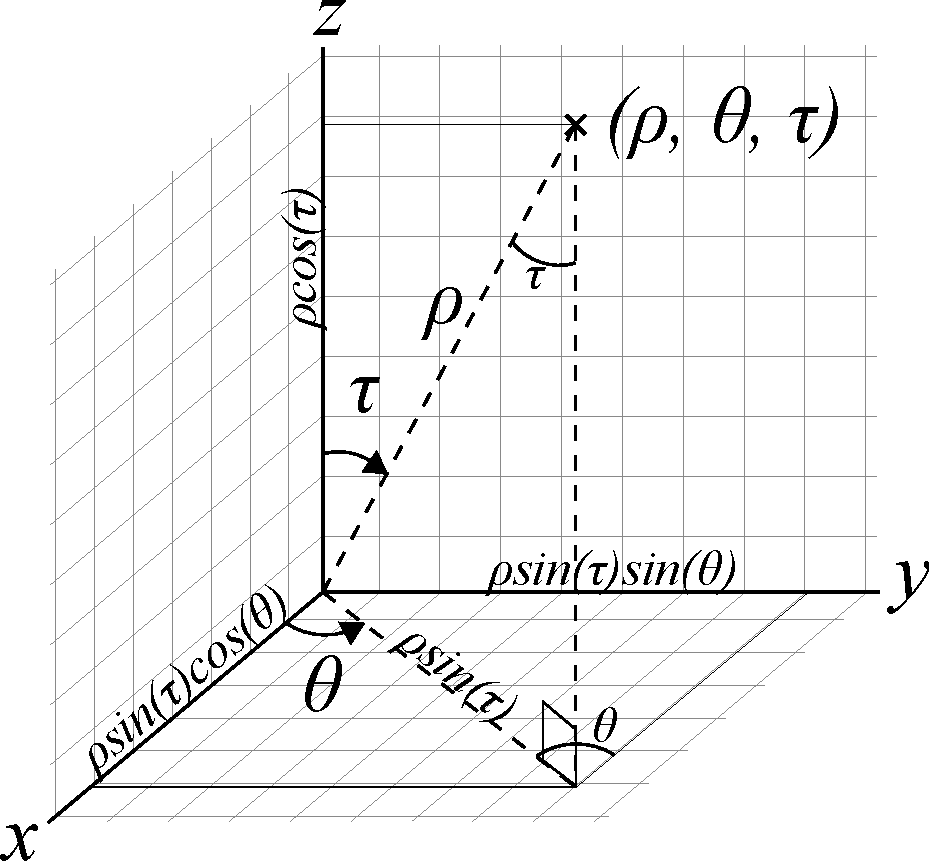
\includegraphics[width=0.5\textwidth]{spherical_coord.pdf}
\end{center}
Come mostrato nella figura, la parametrizzazione sferica di un punto in $\mathbb{R}^3$ è
$$
\varphi (\vartheta,\,\tau) = \left( \cos(\vartheta)\sin(\tau),\, \sin(\vartheta)\sin(\tau),\, \cos(\tau) \right) \qquad (\vartheta,\,\tau) \in [0,\,2\pi] \times [0,\,\pi]
$$
A questo punto, basta procedere come nell'esempio precedente.
\end{example}


\subsubsection{\RNum{2} Metodo: la frontiera di un insieme come vincolo}
\begin{definition}
Un insieme del piano $\mathsf{V} = \lbrace (x,\,y) \in \mathbb{R}^2 : g(x,\,y) = 0 \rbrace$ si chiama \emph{vincolo}.
\end{definition}
Per trattare i vincoli come funzioni, servirà il Teorema delle Funzioni Implicite di Dini. Supponiamo che $A \subseteq \mathbb{R}^2$ aperto e limitato e che $\partial A$ sia un vincolo, ossia $\partial A \lbrace (x,\,y) \in \mathbb{R}^2 : g(x,\,y) = 0 \rbrace$ dove $g \in C^1(\mathbb{R}^2)$. Allora, si può usare il seguente teorema.

\begin{thm}[dei moltiplicatori di Lagrange]
Sia $f \in C^1(\mathbb{R}^2)$ (in realtà non c'è bisogno su tutto $\mathbb{R}^2$!) e sia $g \in C^1(\mathbb{R}^2)$. Supponiamo che $\mathsf{V} = \lbrace (x,\,y) \in \mathbb{R}^2 : g(x,\,y) = 0 \rbrace$ e sia $P_0 = (x_0,\,y_0) \in \mathsf{V}$. Se
\begin{enumerate}[labelindent=\parindent,leftmargin=*,label=\textnormal{(\roman*)},start=1]
\item $\exists \, \underset{\mathsf{V}}{\max} f = f(P_0) \qquad \text{oppure} \qquad \exists \, \underset{\mathsf{V}}{\min} f = f(P_0)$
\item $\nabla g(P_0) \neq (0,\,0)$
\end{enumerate}
allora esiste un $\lambda_0 \in \mathbb{R}$ (detto \emph{moltiplicatore di Lagrange}) per cui il punto $(x_0,\,y_0,\,\lambda_0) \in \mathbb{R}^3$ è un punto stazionario libero della funzione $L : \mathbb{R}^3 \longrightarrow \mathbb{R}$ (detta \emph{funzione lagrangiana}) definita
$$
L(x,\,y,\,\lambda) = f(x,\,y) + \lambda g(x,\,y) \qquad \text{dove} \qquad (x,\,y,\,\lambda) \in \mathbb{R}^3
$$
cioè vale che
$$
\nabla L(P_0) = \left( \frac{\partial f}{\partial x}(P_0) + \lambda_0\frac{\partial g}{\partial x}(P_0),\, \frac{\partial f}{\partial y}(P_0) + \lambda_0\frac{\partial g}{\partial y}(P_0),\, g(P_0) \right) = (0,\,0,\,0)
$$
o, equivalentemente,
\begin{center}
$\mathrm{(\star)}$
\hfill
$\displaystyle
g(P_0) = 0 \qquad \text{e} \qquad \nabla f(P_0) + \lambda_0 \nabla g(P_0) = (0,\,0)
$
\hfill \null \\
\end{center}
\end{thm}

\begin{definition}
Si chiama \emph{punto stazionario vincolato} della funzione $f$ sul vincolo $\mathsf{V}$ un punto $P_0 \in\mathbb{R}^2$ che verifica $\mathrm{(\star)}$.
\end{definition}

Premettiamo, prima della dimostrazione del Teorema di moltiplicatori di Lagrange, il seguente (fondamentale) teorema.

\begin{thm}[delle funzioni implicite, \textsc{U. Dini}]
Siano $g \in C^1(A)$, $A \subseteq \mathbb{R}^2$ aperto, $P_0 = (x_0,\,y_0) \in A$ e supponiamo che
\begin{enumerate}[labelindent=\parindent,leftmargin=*,label=\textnormal{(\roman*)},start=1]
\item $g(P_0) = 0$
\item $\displaystyle \frac{\partial g}{\partial y}(P_0) \neq 0$
\end{enumerate}
Allora
\begin{enumerate}[labelindent=\parindent,leftmargin=*,label=\textnormal{(D\arabic*)},start=1]
\item $\mathsf{V} = \lbrace (x,\,y) \in \mathbb{R}^2 : g(x,\,y) = 0 \rbrace$ è localmente il grafico in un intorno di $P_0$ di una funzione $y = h(x)$, cioè esistono $\delta > 0,\; r_0 > 0$ ed esiste un'unica funzione $h : (x_0 - \delta,\, x_0 + \delta) \longrightarrow \mathbb{R}$ tale che
$$
h(x_0) = y_0
\qquad \text{e} \qquad 
\mathsf{V} \cap \mathrm{B}(P_0,\,x_0) = \lbrace (x,\,h(x) : x \in (x_0 - \delta,\, x_0 + \delta) \rbrace
$$
\item $h$ è di classe $C^1$ su $(x_0 - \delta,\, x_0 + \delta)$ e
$$
h'(x) = - \frac{\displaystyle \frac{\partial g}{\partial x} \left( x,\,h(x) \right)}{\displaystyle \frac{\partial g}{\partial y} \left( x,\,h(x) \right)}
\qquad \forall x \in (x_0 - \delta,\, x_0 + \delta)
$$
\end{enumerate}
\end{thm}

\begin{proof}
(del Teorema dei moltiplicatori di Lagrange)\\
Per il Teorema delle funzioni implicite, esistono $\delta > 0,\; r_0 > 0$ ed una (unica) funzione $h : (x_0 - \delta,\, x_0 + \delta) \longrightarrow \mathbb{R}$ per cui valgono le proprietà (D1) e (D2) se supponiamo, per esempio, $\frac{\partial g}{\partial y}(P_0) \neq 0$.

Consideriamo la funzione $F : (x_0 - \delta,\, x_0 + \delta) \longrightarrow \mathbb{R}$ tale che
$$
F(x) \doteqdot f(x,\,h(x)) \qquad \text{con} \quad x \in (x_0 - \delta,\, x_0 + \delta)
$$
Valendo (i), $x_0$ è un punto di massimo o minimo relativo di $F$ su $(x_0 - \delta,\, x_0 + \delta)$. Per la (RDC), $F$ è di classe $C^1$ su $(x_0 - \delta,\, x_0 + \delta)$ e
$$
F'(x) = \frac{\partial f}{\partial x} (x,\,h(x)) \cdot 1 + \frac{\partial f}{\partial y} (x,\,h(x)) \cdot h'(x) \quad \footnotemark
$$
\footnotetext{
$F = f \circ \gamma$, dove $\gamma (x) = (x,\,h(x))$. Per la (RDC), vale che
$$
F'(x) = \nabla f(\gamma(x)) \bullet \gamma'(x) = \nabla f(x,\,h(x)) \bullet \gamma'(x)
$$
dove $\gamma'(x) = (1,\,h'(x))$
}
Per il Teorema di Fermat (in una variabile),
$$
0 = F'(x_0) =
\frac{\partial f}{\partial x} (P_0) + \frac{\partial f}{\partial y} (P_0) \cdot h'(x_0)
\overset{\mathrm{(D2)}}{=}
\frac{\partial f}{\partial x} (P_0) + \frac{\partial f}{\partial y} (P_0) \cdot 
\left(
- \frac{\displaystyle \frac{\partial g}{\partial x} \left( P_0 \right)}{\displaystyle \frac{\partial g}{\partial y} \left( P_0 \right)}
\right)
$$
moltiplicando tutto per $\frac{\partial g}{\partial y} (P_0)$, otteniamo
$$
0 = 
\frac{\partial f}{\partial x} (P_0) \frac{\partial g}{\partial y} (P_0) -
\frac{\partial f}{\partial y} (P_0) \frac{\partial g}{\partial x} (P_0) =
\det
\left(
\begin{array}{cc}
\frac{\partial f}{\partial x} (P_0) & \frac{\partial f}{\partial y} (P_0)\\
\frac{\partial g}{\partial x} (P_0) & \frac{\partial g}{\partial y} (P_0)
\end{array}
\right)
$$
ossia
$$
\det
\left(
\begin{array}{cc}
\Rigaln{\nabla f(P_0)} \\
\Rigaln{\nabla g(P_0)}
\end{array}
\right)
= 0
$$
In altre parole, $\nabla f(P_0)$ e $\nabla g(P_0)$ sono linearmente dipendenti! Quindi, $\exists \, \lambda_0 \in \mathbb{R}$ tale che valga $\mathrm{(\star)}$.
\end{proof}


\subsection{Interpretazione geometrica della condizione di punto stazionario vincolato}
Dal Teorema di Dini, sappiamo che localmente $\mathsf{V}$ è il grafico di una funzione regolare. Per esempio, nel caso in cui $\frac{\partial g}{\partial y} (P_0) \neq 0$, conosciamo anche l'equazione della retta tangente a $\mathsf{V}$ nel punto $P_0 = (x_0,\,y_0)$. Più precisamente, è la retta di equazione $y = h'(x_0)(x-x_0) + y_0$ dove, da (D2),
$$
h'(x_0) = - \frac{\displaystyle \frac{\partial g}{\partial x} (P_0)}{\displaystyle \frac{\partial g}{\partial y} (P_0)}
$$
La retta tangente è generata (a meno di traslazione) dal vettore $\left( 1,\,h'(x_0) \right)$. Inoltre, vale che
$$
\nabla g(P_0) \bullet \left( 1,\,h'(x_0) \right) = 0
$$
Dunque $\nabla g (P_0)$ è ortogonale alla retta tangente a $\mathsf{V}$ nel punto $P_0$.
\begin{center}
\def\svgwidth{6cm}
\input{./02_massimi_e_minimi/figures/dini_geom.pdf_tex}
\end{center}
Pertanto i punti $P_0 \in \mathsf{V}$ per cui vale $(\star)$ sono i punti $P_0 \in \mathsf{V}$ dove $\nabla f (P_0)$ (e anche $\nabla g (P_0)$, poiché sono linearmente dipendenti) è ortogonale al vincolo $\mathrm{V}$ in $P_0$.

\begin{example}
$f(x,\,y) = x^2 + 2y^2$, $\mathsf{V} = \lbrace (x,\,y) \in \mathrm{R}^2 : x^2 + y^2 = 1 \rbrace$.
Determinare $\underset{\mathsf{V}}{\max} f$ e $\underset{\mathsf{V}}{\min} f$.
\end{example}
\begin{proof}
Applichiamo il metodo dei moltiplicatori di Lagrange. Definendo
$$
g(x,\,y) \doteqdot x^2 + y^2 -1, \qquad (x,\,y) \in \mathbb{R}^2
$$
osserviamo che $f,\,g \in C^{\infty}(\mathbb{R}^2)$, e
$$
\nabla g(x,\,y) = (2x, 2y) = 2(x,\,y) \neq (0,\,0) \qquad \forall (x,\,y) \in \mathsf{V}
$$
Per giungere alla soluzione basta quindi studiare i punti stazionari liberi della funzione lagrangiana
$$
L(x,\,y,\,\lambda) = f(x,\,y) + \lambda g(x,\,y) = x^2 + 2y^2 + \lambda ( x^2 + y^2 -1)
$$
cioè i punti $(x,\,y,\,\lambda) \in \mathbb{R}^3$ tali che
$$
\begin{cases}
\frac{\partial L}{\partial x} (x,\,y,\,\lambda) = 2x + 2\lambda x = 0\\
\frac{\partial L}{\partial y} (x,\,y,\,\lambda) = 4y + 2\lambda y = 0\\
\frac{\partial L}{\partial \lambda} (x,\,y,\,\lambda) = x^2 + y^2 - 1 = 0
\end{cases}
\Longleftrightarrow \quad
\begin{cases}
x = \pm 1\\
y = 0\\
\lambda = -1
\end{cases}
\vee \quad 
\begin{cases}
x = 0\\
y = \pm 1\\
\lambda = -2
\end{cases}
$$
Quindi i punti stazionari vincolati di $f$ su $\mathsf{V}$ sono $(\pm 1,\,0),\;(0,\,\pm 1)$.
\end{proof}

\`E facile generalizzare il metodo dei moltiplicatori di Lagrange ad una funzione di $3$ variabili.

\begin{thm}[dei moltiplicatori di Lagrange]
Sia $f \in C^1(\mathbb{R}^3)$ e sia $g \in C^1(\mathbb{R}^3)$. Supponiamo che $\mathsf{V} = \lbrace (x,\,y,\,z) \in \mathbb{R}^3 : g(x,\,y,\,z) = 0 \rbrace$ e sia $P_0 = (x_0,\,y_0,\,z_0) \in \mathsf{V}$. Se
\begin{enumerate}[labelindent=\parindent,leftmargin=*,label=\textnormal{(\roman*)},start=1]
\item $\exists \, \underset{\mathsf{V}}{\max} f = f(P_0) \qquad \text{oppure} \qquad \exists \, \underset{\mathsf{V}}{\min} f = f(P_0)$
\item $\nabla g(P_0) \neq (0,\,0,\,0)$
\end{enumerate}
allora esiste un $\lambda_0 \in \mathbb{R}$ (detto \emph{moltiplicatore di Lagrange}) per cui il punto $(x_0,\,y_0,\,z_0,\,\lambda_0) \in \mathbb{R}^4$ è un punto stazionario libero della funzione $L : \mathbb{R}^4 \longrightarrow \mathbb{R}$ (detta \emph{funzione lagrangiana}) definita
$$
L(x,\,y,\,z,\,\lambda) = f(x,\,y,\,z) + \lambda g(x,\,y,\,z) \qquad \text{dove} \qquad (x,\,y,\,z,\,\lambda) \in \mathbb{R}^4
$$
cioè vale $\mathrm{(\star)}$.
\begin{center}
\def\svgwidth{10cm}
\input{./02_massimi_e_minimi/figures/lagrange_3d.pdf_tex}
\end{center}
\end{thm}